\documentclass[a4paper]{article}
\usepackage{amsmath}
\usepackage{graphicx}
\usepackage[utf8]{inputenc}
\usepackage[T1]{fontenc}
\usepackage[french]{babel}
\usepackage{amsfonts,amsmath,amssymb}
\usepackage{float}
\usepackage{graphicx}
\usepackage{amsmath}

\title{\textbf{Rapport d'alternance Master 2 Ingénierie logicielle\\ }}
\author{\textbf{MOUTARAJJI} Mouhyi-Eddine\
\\Encadré par :\\\textbf{SALAÜN} Gaël \\\textbf{BOURDÉ} Annabel }
\begin{document}
\date{}

\begin{figure}
\centering

\includegraphics[width=1.1\textwidth]{diagrammes/logoisticfr_0.png}
\end{figure}


\maketitle

\newpage

\tableofcontents
~
\newpage



\section{Rectorat de l’académie de Rennes} 

\subsection{Présentation}

Le rectorat de l'académie de Rennes est une circonscription administrative propre à
l’Éducation Nationale.\\
Elle regroupe 4 directions des services départementaux de l'Éducation Nationale : 
Côtes d'Armor, Finistère, Ille-et-Vilaine et Morbihan. Chaque direction des services départementaux de l'éducation nationale est placée sous la responsabilité d'un inspecteur d'académie, directeur académique des services de l'Éducation nationale.\\\\
Son rôle au sein de ces départements est de gérer les personnels, les élèves, les moyens financiers, les examens... de tous les établissements scolaires, depuis la maternelle jusqu'au lycée.\\\\

\section{L'architecture des projets}

Au sein du rectorat Rennes, la majorité de l'équipe d'informatique  développent des applications web. Il existe plusieurs types d'application (métiers,outils...). Ces applications sont constituées de deux modules. 

\subsection{Back-end}

Le Back-End, c’est la partie du code qui est exécutée par le serveur, il s’agît d'un serveur fournissant une API gérant la persistance des données et la logique de l'application.La majorité des applications du rectorat sont développées en framework Spring-boot et en langage Java et il existe quelques applications développées en langage Kotlin dont l'application Apptour.

L'architecture des projets du rectorat est unique dans tous les projets afin  de faciliter la prise en main de ces derniers et avoir le même point de vue au sein du l'équipe.

Le back-end des applications se décomposent de plusieurs couches: 

une couche Repository/DAO: Repositories sont des interfaces héritant de l'interface Repository. L'objectif de ces interfaces consiste à rendre la création de la couche d'accès aux données (requêtes SELECT, UPDATE...) plus rapide.

une couche Service: Elle permet de séparer les opérations effectuées par le contrôleur et celles qui concernent le modèle des données. Toute action devrait passer par cette couche.

Une couche Contrôller: Il s'agit de l'Api qui permet de répondre à toutes les requêtes envoyées par le client. 

\begin{figure}[H]
	\centering
 		\fbox{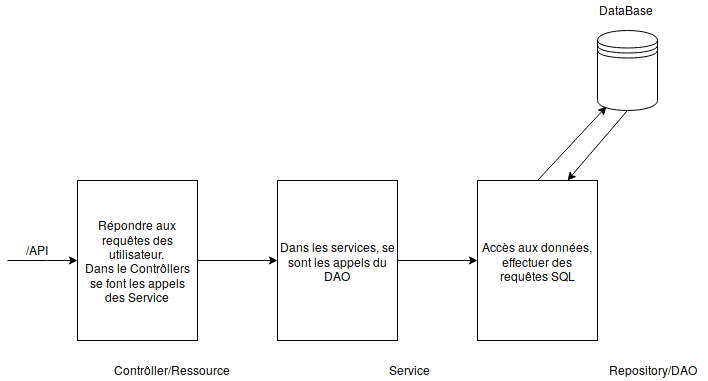
\includegraphics[width=1.2\textwidth]{diagrammes/ArchitectureProjet.png}} 
  		\caption{Arichtecture Back-end d'une application web}
	\end{figure}

\subsection{Front-end}
Le Front-end est la partie visible par les utilisateurs des applications web. Elle comprend l'interface graphique par laquelle nos utilisateurs vont interagir avec 
le reste du système (Back-end).


Le Front-end des applications web du rectorats sont développées en plusieurs langages. La plupart de ces applications  sont codées avec le triplet HTML,CSS \& JavaScript. Tandis que ces derniers mois, l'équipe informatique commence à intégrer le langage React.js  afin de monter en compétences et découvrir des nouveaux langages plus récents. 

\subsubsection{HTML}

HTML est une technologie et un standard qui permet d'afficher le contenu d'une application sur le web. Le langage reprend la syntaxe de XML,c'est-à-dire, une imbrication de balise/élément/tag les uns dans les autres.

\subsubsection{CSS}

CSS, est une technologie complémentaire à HTML, c'est elle qui va permettre d'ajouter des couleurs, des ombres, de mettre en forme le texte, de positionner les blocs, etc. Elle sert à mettre en forme une page web. 

\subsubsection{JavaScript}

JavaScript, au contraire de HTML et CSS, n'est pas un langage de présentation mais de programmation, qui plus est, objet orienté prototype. Il permet de rendre plus dynamique une application web grâce à la manipulation de l'API DOM (Document Object Model) et de l'AJAX (Asynchronous JavaScript And XML).

\subsubsection{React}

Le défaut de JavaScript, mais qui est aussi sa force, est sa grande flexibilité (typage dynamique, première ordre, point virgule optionnel...). On peut donc arriver très facilement à un code illisible et non maintenable. Pour couronner le tout, la DOM est
plutôt quelque chose de difficile à tester. Le framework React apporte beaucoup de solutions à ces problèmes, avec sa façon de manipuler la DOM (via un moteur de template), l'utilisation de TypeScript (une amélioration du JavaScript par Microsoft.De plus, il est très facile de générer un environnement React pour
un projet. C'est pour ces raisons que l'équipe informatique du rectorat commence à prendre en main ce Langage et l’intégrer dans les nouveaux projets et les nouvelles applications web. 

\begin{figure}[H]
	\centering
 		\fbox{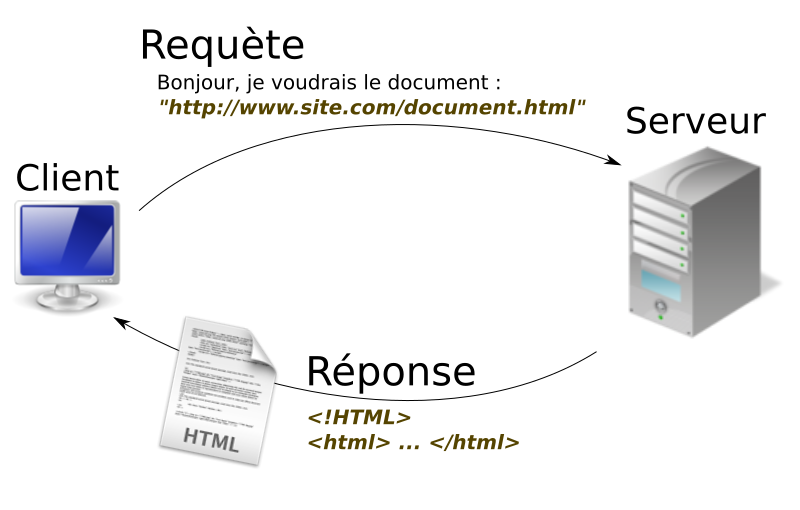
\includegraphics[width=1.2\textwidth]{diagrammes/schema-serveur.png}} 
  		\caption{Application Web classique}
	\end{figure}
 

\end{document}
